\documentclass[final]{beamer}
\mode<presentation>
{
 % \usetheme{collis} 
\usetheme{ANLARM}
}
\graphicspath{{figures/}}
\usepackage{natbib}

\usepackage{times}
\usepackage{amsmath,amssymb}
\usepackage[english]{babel}
\usepackage[latin1]{inputenc}
\usepackage[printwatermark]{xwatermark}
\usepackage[orientation=landscape,size=a0]{beamerposter}  % e.g. custom size poster
\usepackage{tikz}
\addtobeamertemplate{block begin}{\pgfsetfillopacity{0.8}}{\pgfsetfillopacity{1}}

\usebackgroundtemplate{
\tikz\node[opacity=0.5] {\includegraphics[height=\paperheight,width=\paperwidth]{figures/radar2.png}};}


\title{\huge Architectures for Rainfall Property Estimation From Polarimetric Radar}
\author[Collis et al.]{Scott Collis\textsuperscript{1} {\texttt{scollis@anl.gov}},
 Scott Giangrande\textsuperscript{2},
  Jonathan Helmus\textsuperscript{1}
   and Silke Troemel\textsuperscript{3}}
\institute[Argonne]{
1: Argonne National Laboratory Argonne, IL United States \\
2: Brookhaven National Laboratory, Upton, NY United States\\
3: Meteorologisches Institut der Universit{\"a}t Bonn, Bonn, Germany}
\date{\today}

\begin{document}
\begin{frame}{} 
 \begin{columns}[t]
    \begin{column}{.3\linewidth}
  \vfill
  %%%%%%%%%%%Intro Block %%%%%%%%%%%%%%%%%%%%%%%%
      \begin{block}{Introducton}
        \begin{columns}[t]
          \begin{column}{.5\linewidth}
          %%%%%%%%%%%%%%%Col 1: Text%%%%%%%%%%%%%%%%%%%%
        \begin{itemize}
        \item Numerical simulations of decadal climate are done at resolutions far courser than the natural scale of precipitation. 
                 To even have a chance of understanding future precipitation extremes we must reconcile the relation between the statistics of broad-scale
                 precipitation and high resolution observations. 
        \item To this end The Department of Energy's ARM Climate Research Facility operates a network of 5 and 3 cm scanning radar systems. 
        \item Fixed sites are at the Azores, Barrow on the North Slope of Alaska and a multi-scale heterogeneous network on the Southern Great Plains of Oklahoma.                             
         \end{itemize}
         \end{column}
          \begin{column}{.5\linewidth}
          %%%%%%%%%%%%%%%%Col 2: Figure%%%%%%%%%%%%%%%%%%%
           \vskip0ex
            \centering    
           \includegraphics[width=0.95\linewidth]{figures/sgp_layout.png}\\[1ex]            
          \end{column}
         \end{columns}
         \end{block}
         
         
        \begin{block}{Achieving insight with the community: The \textcolor{red}{Py}thon \textcolor{red}{A}RM \textcolor{red}{R}adar \textcolor{red}{T}oolkit}
                \begin{columns}[t]
                    \begin{column}{.55\linewidth}
                        \begin{itemize}
                            \item Weather radars are not a new invention, first academic mention in \citet{bent_radar_1943}.
                            \item Massive advances in computing and radar software has not kept up.
                            \item They Python ARM Radar Toolkit, Py-ART  is a data model driven architecture for interactively and 
                            offline processing of active remote sensing data. Open source and, using GitHub, community based.
                            \item Part of a larger growing international community of codes, see \citet{heistermann_emergence_2014}
                            \item Twenty four forks, eight active contributors from multiple agencies and nations. Broad user base. 
                             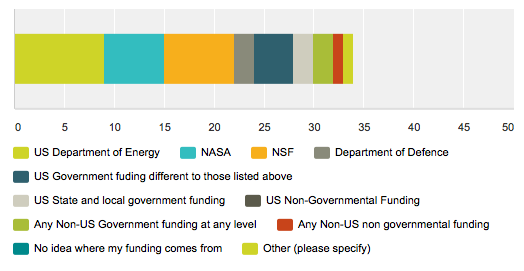
\includegraphics[width=0.8\linewidth]{figures/survey}\\[1ex]                        
                       \end{itemize}
                   \end{column}
                   \begin{column}{.45\linewidth}
                   \vskip0ex
                       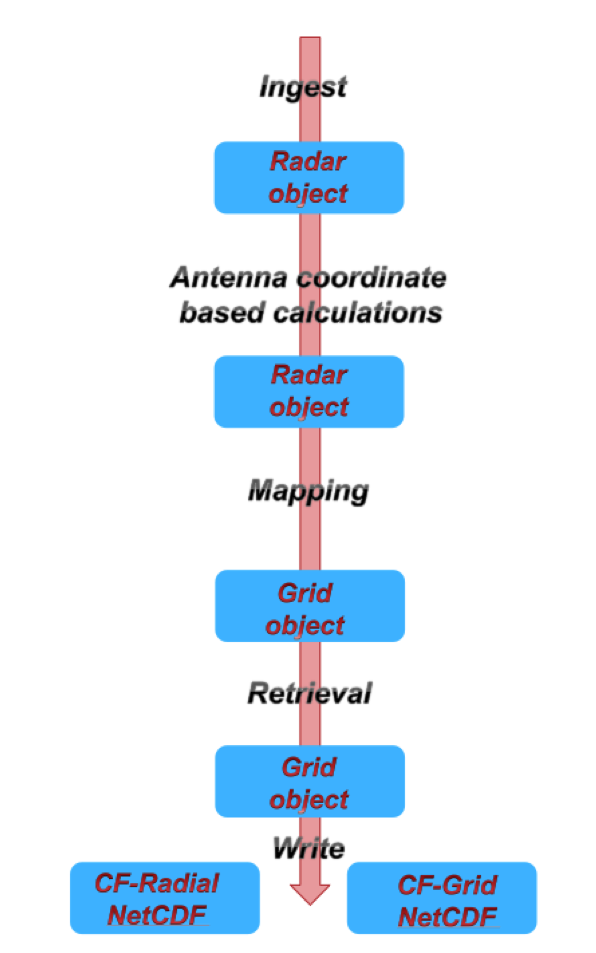
\includegraphics[width=0.9\linewidth]{figures/pyart-flow}\\[1ex]   
                   \end{column}
               \end{columns}
                       \end{block}
        
         \begin{block}{Links}
         	\begin{columns}[c]
	\begin{column}{.02\linewidth}
	\end{column}
         		\begin{column}{.28\linewidth}
		   		\\
         			
         			{\small \hyperlink{http://arm-doe.github.io/pyart/}{The Python ARM Radar Toolkit:}} 
			        \includegraphics[width=.9\linewidth]{figures/python-logo}\\[1ex]   

         	
         		\end{column}
         		\begin{column}{.2\linewidth}
		                 \vskip0ex
		 		
\includegraphics[width=.9\linewidth]{figures/pyart_qr}\\[1ex]   
        		 	\end{column}
			\begin{column}{.3\linewidth}
		   		\\
         			{\small \hyperlink{http://github.com/scollis/AGU_2014_poster/}{This is an open source poster, for notebooks, code and tex:}} 
         	       \includegraphics[width=.376\linewidth]{figures/fork-me-github} \includegraphics[width=.4\linewidth]{figures/scipy} 
         		\end{column}
         		\begin{column}{.2\linewidth}
		                 \vskip0ex
		 		
\includegraphics[width=.9\linewidth]{figures/git_repo_qr}\\[1ex]   
        		 	\end{column}
         	\end{columns}
         \end{block}

  		

    \end{column}
   %COL 2%
      \begin{column}{.3\linewidth}
  \vfill
 
     \begin{block}{Raw data to Quantitative Precipitation Estimates}
 	\begin{columns}[t]
		\begin{column}{.38\linewidth}
		\begin{itemize}
		\item Raw collected radar data in engineering units is unsuitable for comparison with model data. 
		\item Shorter wavelength radar have a higher attenuation cross section. However Signal to noise in phase information much higher and calibration insensitive.
		\item Measured phase is a mix of propagation phase, phase shift on backscatter and artifacts: {\tiny $\phi_{dp}^{signal}(r) = \phi_{dp}^{prop}(r) + \delta(r) + E(r)$}.
		\item When calculating Specific Differential Phase, {\small $K_{dp}$} only the propagation component should be considered, {\tiny $K_{dp} = \frac{d\phi_{dp}^{prop}(r)}{dr}$}.
		\item Method of \citet{giangrande_application_2013} used to extract {\small $\phi_{dp}^{prop}$} and a 20 point sobel filter 
		{\tiny$K_{dp} = \phi_{dp}^{prop} \ast f_{20} = \sum\limits_{M=0}^{19}   \phi_{dp}(r-M)f(M)$} where $f(M)$ is a linear ramp through zero. 
		
		\end{itemize}
		\end{column}
                \begin{column}{.62\linewidth}
                \begin{columns}[t]
                \begin{column}{.5\linewidth}
                		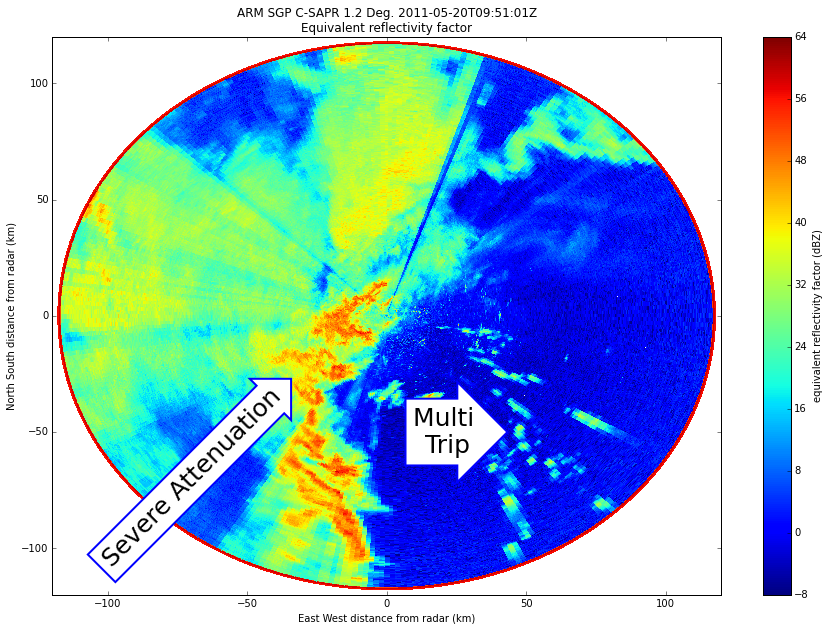
\includegraphics[width=.95\linewidth]{figures/ze.png}\\[1ex]  %r1
           		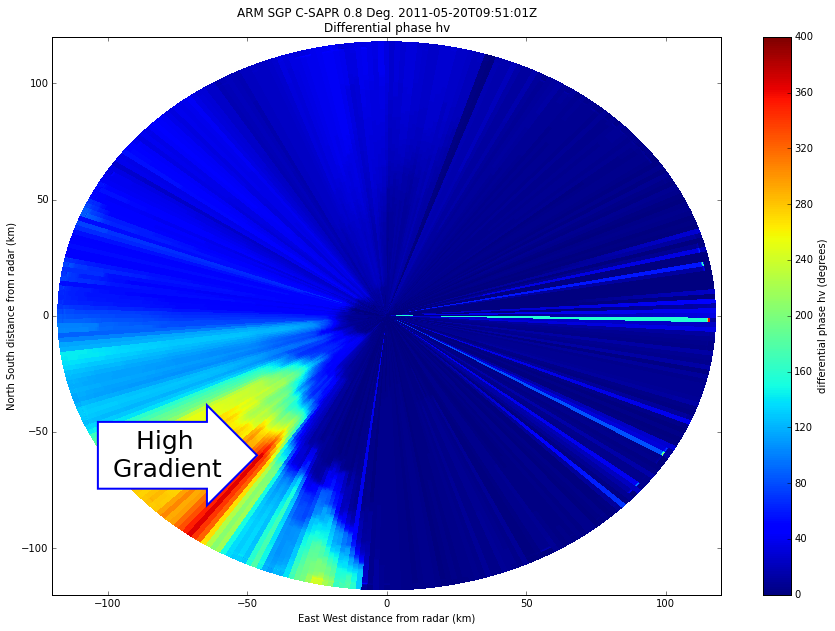
\includegraphics[width=.95\linewidth]{figures/phidp_f.png}\\[1ex]   %r2 
			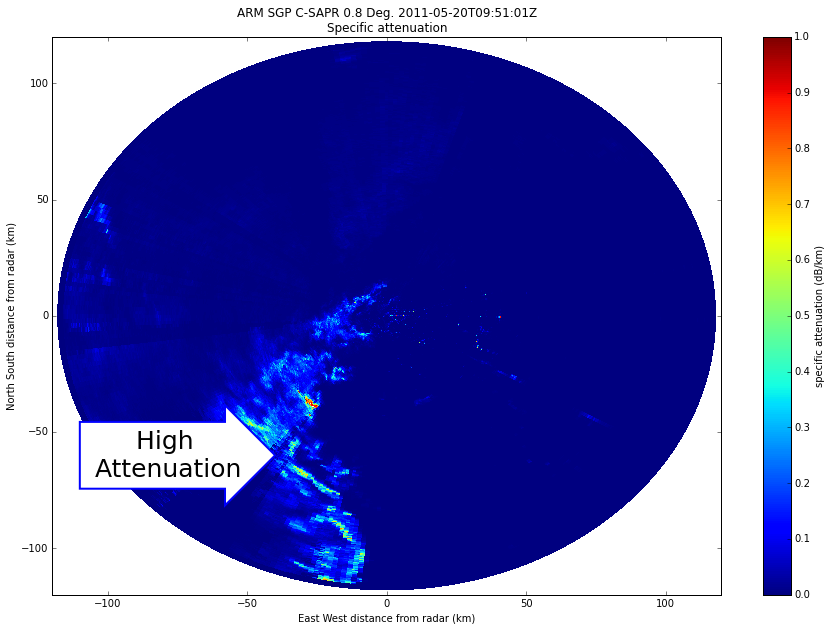
\includegraphics[width=.95\linewidth]{figures/speca.png}\\[1ex]  
		\end{column}
		 \begin{column}{.5\linewidth}
                		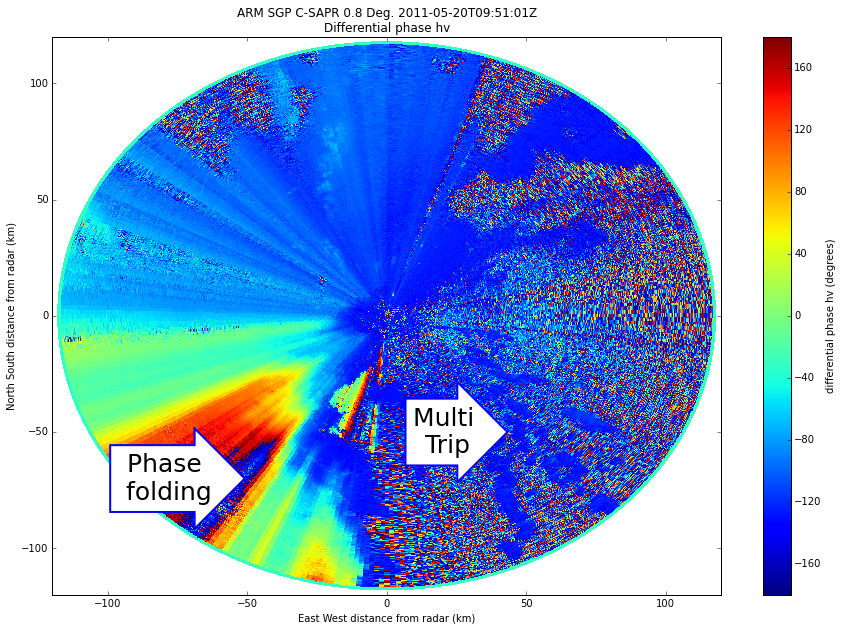
\includegraphics[width=.95\linewidth]{figures/phidp.png}\\[1ex] %r1
           		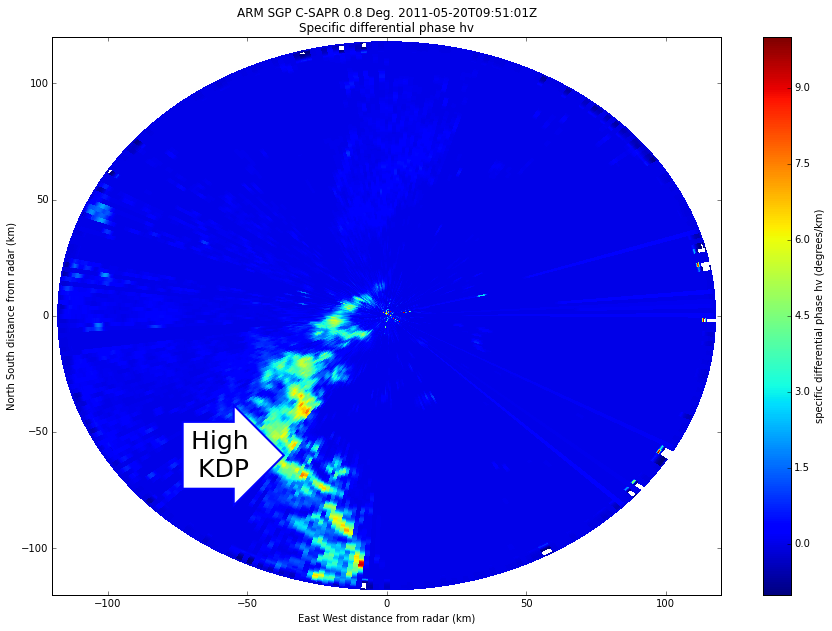
\includegraphics[width=.95\linewidth]{figures/kdp.png}\\[1ex]    %r2
			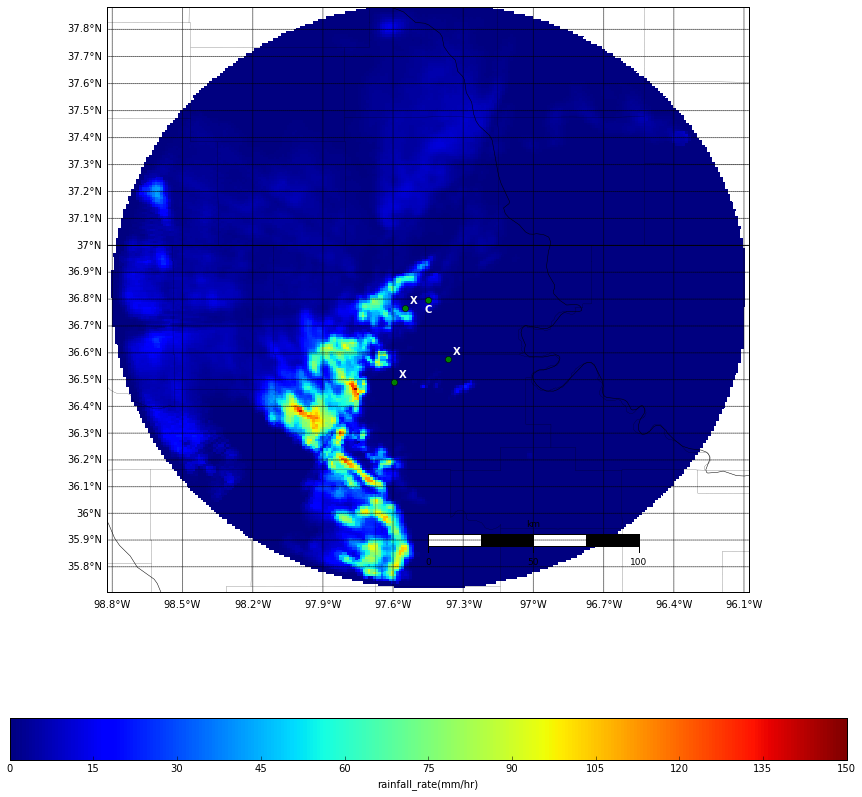
\includegraphics[width=.95\linewidth]{figures/qpe.png}\\[1ex]  
		
		\end{column}
		\end{columns}
 		\end{column}
	\end{columns}
	\begin{itemize}
	\item Specific attenuation is calculated using {\small $K_{dp}$} and {\small $Z_e$} using a method after \citet{gu_polarimetric_2011} and is used as a an estimator for rainfall 
		using a method after \cite{ryzhkov_potential_2014}.
	\item In \citet{giangrande_precipitation_2014} it was shown that specific attenuation at short wavelengths performed as well as retrievals at S-band wavelengths.
	\end{itemize}
      \end{block}
      
      
       \begin{block}{Mapping: Objective analysis}
       \begin{columns}[t]
		\begin{column}{.5\linewidth}
		\begin{itemize}
		\item Radar data is on , $\theta$ and $\phi$ coordinates, there is a need to estimate on different coordinates systems (Cartesian, Sigma, pressure).
		\item Py-ART tags each gate with an estimate of its central coordinate and inserts these into a cloud. 
		\item For propagation insensitive variables (not radial velocity or $\phi_{dp}$), gates can be drawn from mulitple radars to be estimated onto a single grid. 
		
		\end{itemize}
		\end{column}
		\begin{column}{.5\linewidth}
		\vskip0ex
		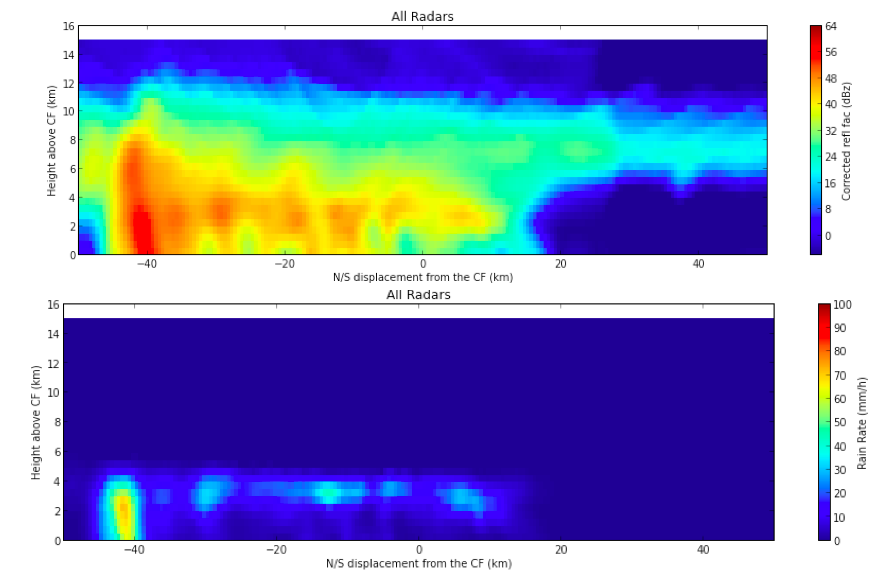
\includegraphics[width=1.0\linewidth]{figures/mapping.png}\\[1ex]     
		\end{column}
	\end{columns}
	\begin{itemize}
	\item In Py-ART the act of gridding takes in a {\it n-tuple} of radar objects and returns a grid object which can be saved to a CF-Radial complaint file.
	\end{itemize}	
	\includegraphics[width=.95\linewidth]{figures/code}\\[1ex]   

         \end{block}


    \end{column}
%COL 3%
  \begin{column}{.3\linewidth}
  \vfill
   \begin{block}{Advective interpolation}
 	\begin{columns}[t]
		\begin{column}{.6\linewidth}
		\begin{itemize}
		\item Simply accumulating precipitation retrievals by integrating can create a "chain of pearls effect" due to the lack of spatial coherency between successive radar scans.
		\item This can create false information and skew any interpretation of the scale of rainfall.
		\item The solution is to calculate the image advection and then generate sub-temporal-scale images and average:
		
		\small
		\begin{align*}
                G(t + \Delta{}t, z, y, x) &= (1 - \frac{t + \Delta{}t - t_1}{t_2 - t_1})G_1(t_1, z, y + v\Delta{}t, x + u\Delta{}t) \\
                                             &+ \frac{t + \Delta{}t - t_1}{t_2 - t_1}G_2(t_2, z, y - v\Delta{}t, x - u\Delta{}t)
                \end{align*}
                \normalsize
               \item Setting $t_1 = 0$
               \small
                \begin{align*}
                G(t + \Delta{}t, z, y, x) &= (1 - \frac{t + \Delta{}t}{t_2 })G_1(t_1, z, y + v\Delta{}t, x + u\Delta{}t) \\
                                             &+ \frac{t + \Delta{}t}{t_2}G_2(t_2, z, y - v\Delta{}t, x - u\Delta{}t)
                \end{align*}
                \normalsize
                \item In a nice novel twist (we Py-ART developers love applying math to radar) the advection can be determined from the cross correlation phase between the two images, 
                $r = \mathcal{F}^{-1}\left\{C\right\}$.
                \item Borrowing liberally from \hyperlink{http://en.wikipedia.org/wiki/Phase_correlation}{Wikipedia}: 
                	\small
		\begin{gather*}
		\boldsymbol{G}_{t1} = \mathcal{F}\left\{R_{t1}\right\}, \boldsymbol{G}_{t2} = \mathcal{F}\left\{R_{t2}\right\}\\
		C = \frac{\boldsymbol{G}_{t1}\circ\boldsymbol{G}^*_{t2}}{\left|\boldsymbol{G}_{t1}\circ\boldsymbol{G}^*_{t2}\right|}\\
		r = \mathcal{F}^{-1}\left\{C\right\}\\
		\Delta{}x, \Delta{}y = \mathrm{argmax}\left\{r\right\}
				\end{gather*}
		\normalsize

            
                \end{itemize}
		\end{column}
                \begin{column}{.4\linewidth}
            
                \vskip0ex
           		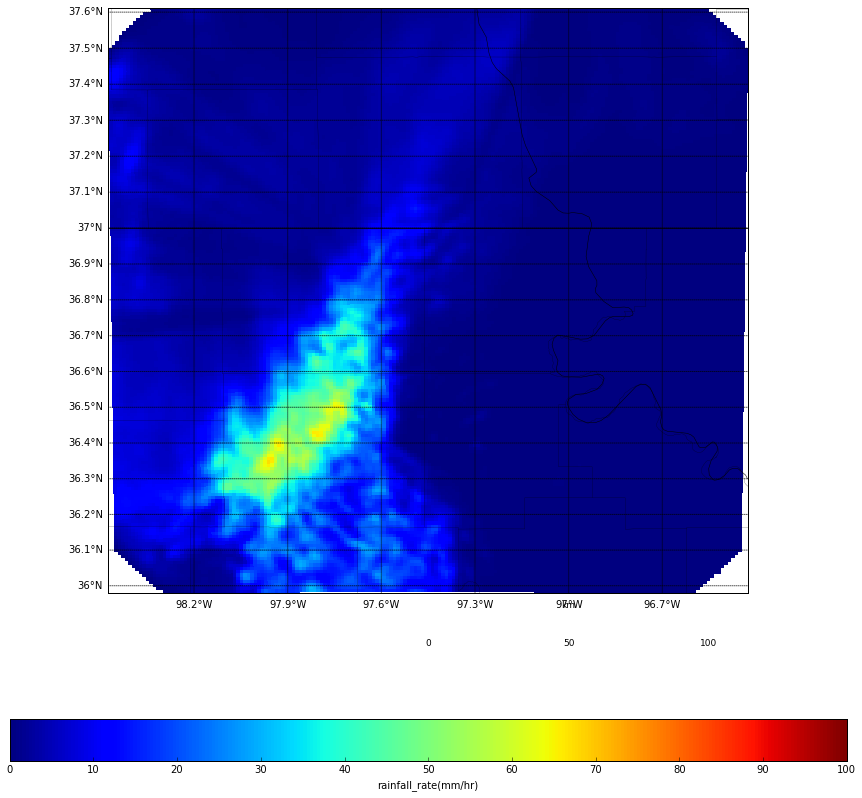
\includegraphics[width=1.0\linewidth]{figures/basic_accumulation.png}\\[1ex]     
            		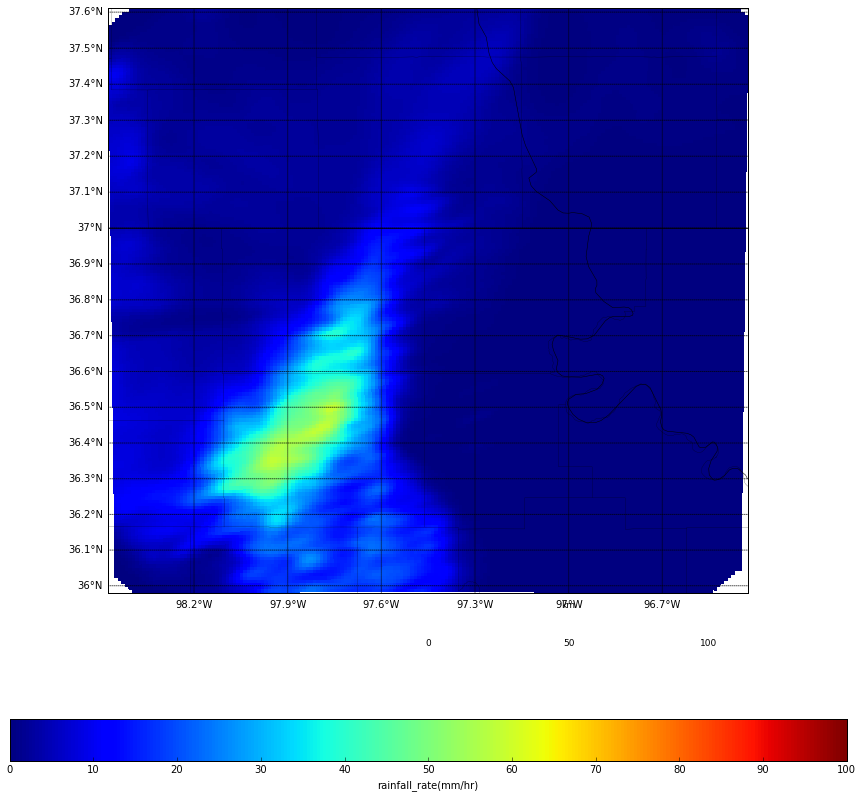
\includegraphics[width=1.0\linewidth]{figures/advective_accum.png}\\[1ex]  
 		\end{column}
	\end{columns}
	      \begin{itemize}
	      \item where $\mathcal{F}$ is the Fourier transform, $^*$ is the complex conjugate and $\circ$ represents element wise multiplication. 
	      \item Summing sub-sample advective interpolation steps results in an accumulation that is less effected by lack of temporal resolution.
	      \item As an added bonus this technique can be used the temporal resolution in point estimates by effectively projecting the spatial to the temporal dimension.
                \end{itemize}

      \end{block}
   
   
        \begin{block}{References}
        \small
       \bibliographystyle{ametsoc}
       \bibliography{zotero} 
         \end{block}


    \end{column}

  \end{columns}


  \vfill
\end{frame}
\end{document}


%%%%%%%%%%%%%%%%%%%%%%%%%%%%%%%%%%%%%%%%%%%%%%%%%%%%%%%%%%%%%%%%%%%%%%%%%%%%%%%%%%%%%%%%%%%%%%%%%%%%
%%% Local Variables: 
%%% mode: latex
%%% TeX-PDF-mode: t